\section{Proposal}



\subsection{Description}

\begin{description}
    \item Protocol : Ethernet
    \item MAC protocol : CSMA / CD
    \item Computer language : JavaScript, HTML5
    \item Platform : ALL
\end{description}

\subsection{The high-level description of the simulation algorithm}


\begin{center}
\item Algorithm for CSMA /CD
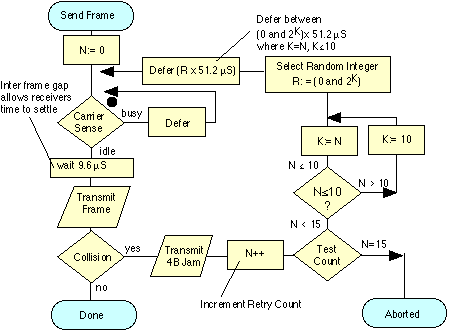
\includegraphics[scale=0.8]{ether.png}
\end{center}

\newpage

\subsection{The mathematical formulae}

\subsubsection{Synchronous data traffic}
Packet arrival and inter arrival time are all uniform and deterministic.
\begin{description}
    \item Arrival process : packet size / bandwidth ( packets/sec)
    \item Traffic load = packet arrival time rate * packet size
    \item Average packet delay = transmission time for one packet
    \item Delay Variance = 0 because intervals are equal.
    \item Thoughput = $\frac{number of byte sent}{total time}$
\end{description}

\subsubsection{Asynchronous data traffic}

\begin{description}
    \item Arrival process : $ \frac{e^{b} \cdot b^{k}}{k!}$ (Poisson distribution)
    \item Traffic load = packet arrival time rate  (Poisson distribution : $ \frac{e^{b} \cdot b^{k}}{k!}$) $\times$ packet size (Exponential distribution : $\lambda \cdot e^{ \lambda \cdot t}$)
	\begin{description}  
    \item b = $\lambda \cdot$t
    \item t is used to define the interval 0 to t   
    \item $\lambda$ is the total average arrival rate in packets
   	\item k is the total number of packets in the interval 0 to t
   	\end{description}
    \item Average packet delay = $\overline{x} = \dfrac{1}{n} \sum_{i=1}^{n} x_{i}$
    \item Delay Variance = $ V(X) = \dfrac{1}{n} \sum_{i=1}^{n} x_{i}^{2} - \overline{x}$
    	\begin{description}
    	\item X : Delay
    	\item n = number of packets
    	\item $x_{i}$ = delay for packet number \begin{tiny}
•
\end{tiny}i
    	\item $\overline{x}$ = average packet delay
       	\end{description}
    \item Thoughput = $\frac{number of byte sent}{total time}$
\end{description}

\subsection{The list of references}
\begin{description}
\item Chapter 2 of the textbook by Peterson and Davie
\item The set of handout on simulation provided.
\item \href{http://mathworld.wolfram.com/PoissonDistribution.html}{http://mathworld.wolfram.com/PoissonDistribution.html}
\item \href{http://www.erg.abdn.ac.uk/~gorry/eg3561/lan-pages/csma-cd.html}{http://www.erg.abdn.ac.uk/~gorry/eg3561/lan-pages/csma-cd.html}
\end{description}

